\documentclass{article} % Change to a standard article class
\usepackage{amsmath} % for math environments and commands
\usepackage{cite}
\usepackage{amssymb}
\usepackage{amsfonts}
\usepackage{graphicx}
\usepackage{textcomp}
\usepackage{xcolor}

\begin{document}

\title{SVM - Support Vector Machine\\
\thanks{Insert applicable funding agency here. If none, delete this.}
}

\author{Arthur Felipe Reis Souza \\
Electrical Engineering Department, \\
Federal University of Minas Gerais, \\
Belo Horizonte, Brazil \\
arthurfreisouza@gmail.com \\
\and
Antônio de Pádua Braga and Frederico Gualberto Ferreira Coelho \\
Electrical Engineering Department, \\
Federal University of Minas Gerais, \\
Belo Horizonte, Brazil \\
apbraga@cpdee.ufmg.br, fredgfc@ufmg.br
}

\maketitle

\begin{abstract}

    Esse relatório tem por objetivo demonstrar o algoritmo de Machine Learning Support Vector Machine (SVM), suas vantagens, desvantagens e aplicações.

\end{abstract}

\section{Introdução}

O algoritmo Support Vector Machine (SVM) é amplamente utilizado em Machine Learning tanto para tarefas de classificação quanto de regressão, sendo mais comumente utilizado para classificação. No contexto de classificação esse algoritmo é um separador que consiste em maximizar a margem entre a reta separadora e os vetores de suporte. Os vetores de suporte são os pontos de cada classe que estão mais próximos do separador, sendo eles os pontos que mais importam na hora de realizar a classificação, podendo ignorar todo o restante.

\vspace{1cm}

\begin{figure}[h] % 'h' posiciona a figura aproximadamente no local do código
    \centering % centraliza a figura
    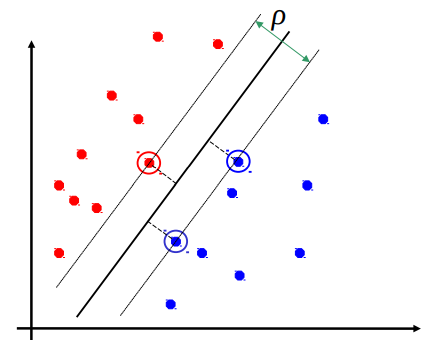
\includegraphics[width=0.5\linewidth]{SVM_pic.png} % insira o caminho da sua imagem e ajuste a largura
    \caption{Margens de uma SVM, com sua reta separadora.} % insira a legenda desejada
    \label{fig:exemplo} % rótulo para referenciar a figura no texto
\end{figure}

\vspace{1cm}

Esse algoritmo é um separador linear, por natureza, e não pode separar claramente duas classes que são não linearmente separáveis. Para isso, usa-se uma função de kernel que leva esses pontos não separáveis para uma outra dimensão onde os mesmos são separáveis por uma reta ou um hiperplano N-dimensional. Há várias funções de kernel que podem ser utilizadas, e dependerá de cada situação de aplicação

\vspace{1cm}

\begin{figure}[h] % 'h' posiciona a figura aproximadamente no local do código
    \centering % centraliza a figura
    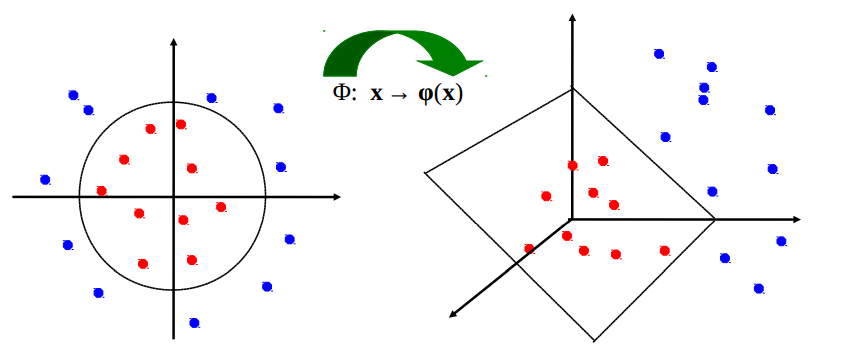
\includegraphics[width=0.75\linewidth]{Kernel_SVM.png} % insira o caminho da sua imagem e ajuste a largura
    \caption{Função de Kernel levando os pontos para outra dimensão.} % insira a legenda desejada
    \label{fig:exemplo} % rótulo para referenciar a figura no texto
\end{figure}

\vspace{1cm}

Outro fator influente nesse algoritmo é se ele possui uma "soft-margin" ou uma "hard-margin". Esses conceitos serão melhores esclarescidos ao decorrer do relatório, mas de maneira resumida esses tipos de margem tem relação com o tradeoff entre o bias (erro nos dados de treino) e o termo variance (erro nos dados de teste) do modelo. Portanto, controlando a margem com o hiperparametro C, podemos controlar o overfitting do modelo.

\section{Geração dos dados}

\vspace{1cm}

Os dados foram gerados com base em distribuições espirais, conjunto de dados cuja característica é ser não linearmente separável. A ideia é construir um classificador do tipo SVM para separar ambos os conjuntos, tendo um bom desempenho tanto para os dados de treino quanto para os dados de teste, variando o hiperparametro C.

\vspace{1cm}

\begin{figure}[h] % 'h' posiciona a figura aproximadamente no local do código
    \centering % centraliza a figura
    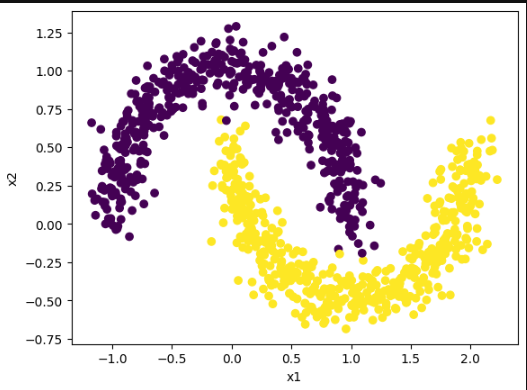
\includegraphics[width=0.5\linewidth]{spiral_plot.png} % insira o caminho da sua imagem e ajuste a largura
    \caption{Conjunto de dados espiralS.} % insira a legenda desejada
    \label{fig:exemplo} % rótulo para referenciar a figura no texto
\end{figure}

\vspace{1cm}

É notório acima que as classes são não linearmente separáveis. Para deixá-las separáveis, usaremos os kernels em um Grid e testar cada combinação, pegando o kernel que resultar em uma melhor acurácia.

\vspace{1cm}

\section{Desenvolvimento}

\vspace{1cm}

A função do SVM está incluída na biblioteca scikit-learn em Python, eliminando a necessidade de implementá-la do zero. No exercício, foi realizada uma busca em grade (grid search), que identificou o kernel "rbf" como o mais adequado para a base de dados. Em seguida, utilizando esse kernel, variou-se o hiperparâmetro C para analisar o desempenho do modelo.

\vspace{1cm}

\section{Resultados e Discussão}

\vspace{1cm}

As duas imagens abaixo representam a superfície de separação para o modelo ao variar C. Note-se que para C = 1,a superfície de separação do modelo é mais suave, indicando que ele generaliza melhor para essa situação. No entanto, ao utilizar C = 150, um valor bastante elevado, podes-se concluir tendencias de overfitting.

\vspace{1cm}

\begin{figure}[h] % 'h' posiciona a figura aproximadamente no local do código
    \centering % centraliza a figura
    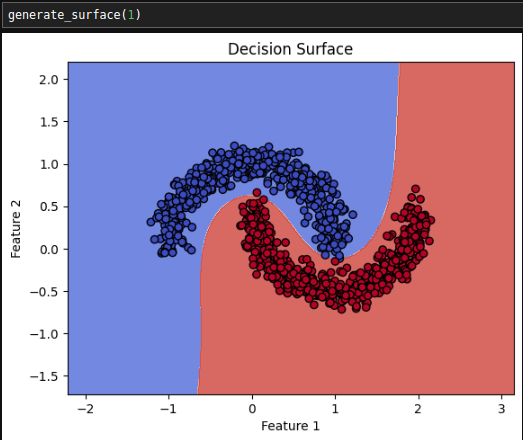
\includegraphics[width=0.5\linewidth]{svm_c_1.png} % insira o caminho da sua imagem e ajuste a largura
    \caption{SVM com C = 1.} % insira a legenda desejada
    \label{fig:exemplo} % rótulo para referenciar a figura no texto
\end{figure}

\vspace{1cm}

\begin{figure}[h] % 'h' posiciona a figura aproximadamente no local do código
    \centering % centraliza a figura
    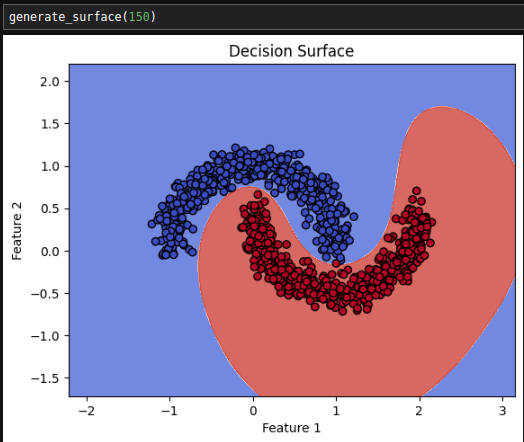
\includegraphics[width=0.5\linewidth]{svm_c_150.png} % insira o caminho da sua imagem e ajuste a largura
    \caption{SVM com C = 150.} % insira a legenda desejada
    \label{fig:exemplo} % rótulo para referenciar a figura no texto
\end{figure}

\vspace{1cm}

Aprofundando na lógica do hiperparâmetro C: A principal ideia por trás de uma SVM (Máquina de Vetores de Suporte) é maximizar a margem entre a reta separadora e os vetores de suporte. Para isso, é necessário controlar o módulo dos pesos \( w \) da reta separadora, limitando-os. Como mostrado na equação abaixo, ao introduzir o hiperparâmetro C, temos a liberdade de ajustá-lo para controlar o overfitting do modelo. Um valor elevado de C implica que menos amostras \( \epsilon \) serão consideradas como erros de classificação. Cada amostra \( \epsilon \) corresponde a um erro de classificação, ou seja, uma amostra que foi classificada incorretamente. Ao aumentar ou diminuir o número de amostras classificadas erroneamente, estamos ajustando a margem do modelo. Um valor alto de C resultará em menos erros de classificação \( \epsilon \), levando a uma margem menor (hard margin). Por outro lado, um valor baixo de C permitirá mais erros de classificação, ampliando a margem do modelo (soft margin).

\vspace{1cm}

\begin{figure}[h] % 'h' posiciona a figura aproximadamente no local do código
    \centering % centraliza a figura
    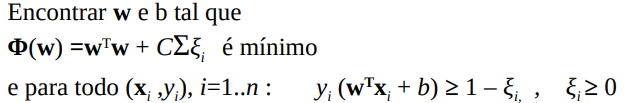
\includegraphics[width=0.75\linewidth]{math_svm.png} % insira o caminho da sua imagem e ajuste a largura
    \caption{Matemática para o valor de C.} % insira a legenda desejada
    \label{fig:exemplo} % rótulo para referenciar a figura no texto
\end{figure}

\vspace{1cm}

\section{Conclusão}

Portanto, ao finalizar o exercíco é possível observar e estudar o algoritmo SVM- Support Vector Machine, é possível analisar como a superfície de separação e o classificador é fortemente afetada pelo hiperparametro C, onde quando C tem um valor elevado o modelo tende ao overfitting e quando C tem um valor baixo o modelo tende a uma melhor generalização, pois C controla a margem e o overfitting do modelo. Uma boa lógica para escolher os valores de C é através por algoritmos de teste como o GridSearch.

\end{document}